\section{Jackson und das Jackson Projekt}\label{Jackson}
Das Jackson-Projekt entwickelt eine freie und modulare Bibliothek f\"ur die Serialisierung und Deserialisierung von Java-Instanzen in \ac{JSON}-Dokumente und zur\"uck. Jackson wird unter der Contributor License Agreement (CLA) vermarktet. Die zur Zeit aktuelle Version ist 2.4.1, welche auch bei der Bearbeitung des Projektes eingesetzt wird.

\subsection{Jackson-Module}
Die Jackson-Bibliothek besteht aus drei Hauptmodulen, welche wie folgt bezeichnet sind:
\begin{itemize}
 \item "`jackson-core"' welches die JSON spezifische Implementierung sowie eine low-level streaming API enth\"alt 
 \item "`jackson-databind"' welches f\"ur das \textit{databind} verantwortlich ist.
 \item "`jackson-module-jsonSchema"' welches ein JSON-Schema f\"ur eine Klasse erstellt
 \item "`jackson-annotations"' welches die Jackson spezifischen Annotationen enth\"alt.
 \item "`jackson-module-jaxb-annotations"' ist f\"ur die Verarbeitung von JAXB-Annotationen verantwortlich
\end{itemize}
Der Core enth\"alt die low-level-streaming API welche die Kommunikation zwischen den einzelnen Modulen \"ubernimmt. Des weiteren enth\"alt dieses Modul viele Grundklassen die auch in anderen Modulen ben\"otigt werden.

Die Jackson Annotationen enthalten Informationen die f\"ur das Serialisieren beziehungsweise Deserialisieren verantwortlich sind.
Jackson kann aber auch Annotationen von anderen Serialisierern erkennen und darauf reagieren.

Eine Mischung von Annotationen von verschiedenen Serialisierern ist Grunds\"atzlich m\"oglich, aber nicht empfehlenswert da hier die \"Ubersichtlichkeit und die Verst\"andlichkeit des Codes leidet.

Unter Databind wird eine Methode verstanden, welche \"uber ein Userinterface gesteuert werden kann.
Dieses Modul ist in der Lage Daten aus einem Datenstrom wie zum Beispiel einem JSON-File zu lesen oder zu schreiben.

Mit diesen drei Modulen ist Jackson voll einsetzbar und kann Java-Instanzen zu einem JSON-Datenstrom umwandeln. Der JSON-Datenstrom wiederum kann gespeichert oder an andere Programme gesendet werden.

Um jedoch einheitliche Annotationen f\"ur Jackson und JAXB zu haben, wird ein weiteres Jackson-Modul ben\"otigt, welches in der Lage ist die JAXB-Annotationen zu verarbeiten.

Auch die Erstellung eines JSON-Schemas aus der Klasse ist mit Hilfe des Moduls "`jackson-module-jsonSchema"' m\"oglich. Wie eine Schemaerzeugung genau funktioniert wird im Kapitel \ref{JSON-Schema} genauer erkl\"art. \cite{Jackson}

\subsection{Serialisierung mit Jackson}\label{Serialisierung}
Der im folgenden beschriebene Sachverhalt erl\"autert das Quellcode-Listing unten.

Um eine Serialisierung mit Jackson umzusetzen wird zuerst eine Instanz der Klasse \\\texttt{ObjectMapper} ben\"otigt, welche den Databinder darstellt, welcher wie schon dargestellt den Datenstrom verarbeitet. Dieser \texttt{mapper} ist somit f\"ur die Convertierung von Java-Instanzen zu JSON-Dokumenten verantwortlich. Das zu serialisierende Objekt ist im Beispiel \texttt{opmObject}, welches der Methode \texttt{serialize} \"ubergeben wird.

Jedoch wird nicht nur der \texttt{mapper} ben\"otigt, sondern auch ein \texttt{AnnotationInspector} der jedoch abstrakt ist. Der \texttt{inspector} wird deshalb als Instanz von \texttt{JaxbAnnotationInspector} erstellt, was durch eine Implementierung der abstrakten Klasse m\"oglich ist. 

Dem \texttt{inspector} wird eine \texttt{TypeFactory} mit "`Default-Einstellungen"' \"ubergeben . Dies bedeutet es wird auf die Original JAXB-Annotationen geparst, ohne auf Sonderf\"alle zu achten. Andere Annotation werden nicht ber\"ucksichtigt. Der \texttt{inspector} wird schlie\ss{}lich, nach der Erstellung, dem \texttt{mapper} \"ubergeben, damit dieser auf die entsprechnden Annotationen reagieren kann.

Um eine \textit{Minimal Exception Safety} zu garantieren wird nun eine \texttt{null}-Abfrage des zu serialisierenden Elements (\texttt{opmObject}) gemacht. Mit dieser Stufe der Sicherheit soll nicht verhindert werden, dass eine Exception passiert. Es wird lediglich garantiert, dass die Methode ohne abzust\"urzen durchlaufen werden kann. \cite{ExceptionSafety}

Ist die zu serialisierende Instanz \texttt{null}, so wird eine \texttt{IllegalagumentException} generiert und die Methode so ordnungsgem\"a\ss{} beendet. Ist eine Instanz vorhanden, wird diese dem \texttt{mapper} \"ubergeben. Das Ergebnis des Aufrufs der Methode \texttt{writeValueAsString} von der Klasse \texttt{ObjectMapper} ist entweder bei Erfolg ein valider JSON-String oder beim Scheitern eine \\\texttt{JsonProcessingException}. 

Eine \texttt{JsonProcessingException} wird generiert, wenn Probleme beim parsen, beziehungsweise beim generieren des JSON-Kontent auftreten die keine puren I/O-Probleme sind. Die Exception erbt jedoch von \texttt{IOExecption}. Bei der \texttt{JsonProcessingException} handelt es sich um eine "`checked"' Exception welche irgendwo im Programmablauf abgefangen werden muss.

\lstinputlisting{Code/Jackson_bsp.java}
\newpage
\subsection{Deserialisierung mit Jackson}
Der im folgenden beschriebene Zusammenhang ist noch einmal im Quellcode-Listing unten zu finden.

F\"ur die Deserialisierung mit Hilfe von Jackson wird wie bei der Serialisierung ebenfalls ein Databinder, also ein Objekt der Klasse \texttt{ObjectMapper} und ein \texttt{AnnotationInspector} ben\"otigt, welche wie im Kapitel \ref{Serialisierung} erstellt werden. 

Bevor dies jedoch passiert, wird gepr\"uft ob der eingegebene String weder \texttt{null} noch \texttt{empty} ist, womit wieder die \textit{Minimal Exception Safety} garantiert werden kann. Sollte einer F\"alle auftreten, so wird eine \texttt{IllegalagumentException} zur\"uckgeliefert.

Wenn der String, wie eigentlich zu erwarten ist, einen Inhalt habt, wird die Methode \texttt{readValue} vom \texttt{mapper} mit dem \"ubergebenden String und der Information um welche Klassen-Instanz es sich beim String handelt \"ubergeben. Der zur\"uckgegebene Typ, der Methode \texttt{readValue}, entspricht dem Typ der im zweiten Argument \"ubergebenen Instanz.

Die Schwierigkeit beim Deserialisieren besteht nun darin, dass bevor der String \"uberhaupt deserialisiert werden kann, erst festgestellt werden muss um welche Klasse es sich eigentlich handelt.

Im Codebeispiel unten wird momentan noch davon ausgegangen, das es sich immer um eine Instanz der Klasse "`TestData"' handelt. Wie diese Einsch\"ankung aufgehoben werden kann, wird im folgenden Kapitel genauer beschrieben.

\lstinputlisting{Code/Jackson_des_bsp.java}

\subsection{Instanzunabh\"angige Deserialisierung}
Wie gerade schon erkl\"autert, wird beim Deserialisieren vorausgesetzt, dass der Typ, der Instanz, des zu deserialisierenden Strings bekannt ist.

Um den String nun eindeutig einem Typ zuzuordnen musste eine eindeutige Kennzeichnung geschaffen werden.

Es wurde sich daraufhin in der Projektgruppe geeinigt, dass ein String der Klassenname \"uber ein Attribut \texttt{className} hinzugef\"ugt wird. Aus diesem Grund bekam die Klasse \texttt{OPMObject} ein String-Attribut \texttt{className} in welchem der Klassenname der jeweiligen Klasse abgelegt ist.

Durch die gemeinsame Wurzelklasse \texttt{OPMObject} haben nun alle Klasse das Attribut \texttt{className} geerbt. 
Daraus ergibt sich wiederum im Umkehrschluss, dass nur noch Klassen welche von \texttt{OPMObject} erben serialisiert werden k\"onnen, da nur sie mit Sicherheit das \texttt{className}-Attribut enthalten.

Beim Serialisieren wird nun der Klassenname mit in den Ausgabe-String geschrieben und dieser kann dadurch eindeutig identifiziert werden.

Um nun den Klassennamen aus den String zu lesen, wurde die neue Methode \\\texttt{getClassFileFromString} geschrieben, welche den Klassennamen aus dem String filtert und diesen dann zur\"uckliefert. Das Auslesen des Typ-Namen wurde, mit Hilfe der \texttt{split}-Methode der String-Klasse realisiert.

\subsection{Klassendiagramm der Serialisierung}

Wie von OPM verlangt erben hier alle Klassen von \texttt{OPMObject}. Um die Geschwindigkeit, beziehungsweise die Funktionalit\"at der XML- und JSON-Serialisierung vergleichen zu k\"onnen wurde eine gemeinsame abstrakte Klasse \texttt{Serializer} generiert. 

Die Klasse \texttt{JSONSerializer} erbt um einen direkten Vergleich durchf\"uhren zu k\"onnen genau wie \texttt{XMLSerializer} von \texttt{Serializer}.
\texttt{Testdata} und \texttt{TestData2OPM} sind erste Test-Klassen von denen Instanzen serialisiert und deserialisiert werden.
Main-Klasse in diesem Projekt ist \texttt{OPM\_Serializer}. Die \texttt{main}-Methode setzt die Serialisierung zum testen in Gang.

Damit wie gew\"unscht jede Klasse serialisiert werden kann, wurde die Methode \texttt{serializeMe} zu OPMObject hinzugef\"ugt. Der Methode muss eine Instanz des Serialisierers \"ubergeben werden, welcher f\"ur die Serialisierung genutzt werden soll.

Durch die Vererbung im OPM-Modell, erbt jede Klasse die Methode \texttt{serializeMe}.
Diese Methode nutzt nun bei Aufruf die \texttt{serialize}-Methode des jeweiligen Serialisierers um die Serialisierung durchzuf\"uhren.

Ein vollst\"andiger \"Uberblick ist im Klassendiagramm auf der n\"achsten Seite zu finden.


\begin{figure}[ht]
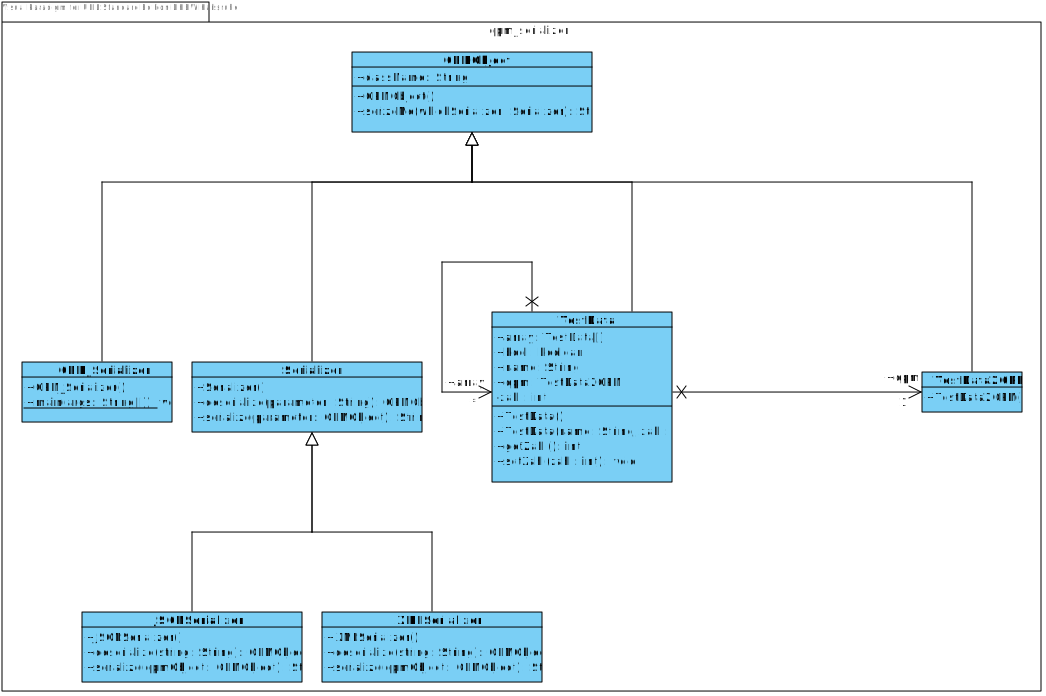
\includegraphics[width=16cm]{Bilder/Erstes_EKD}
\label{Klassendiagramm der Serialisierung}
\caption{Klassendiagramm der Serialisierung} 
\end{figure}
\FloatBarrier
\subsection{JSON-Schema Erstellung aus einer Klasse}\label{JSON-Schema}
\"Ahnlich wie auch bei XML gibt es in JSON ein Datenformat, welches die zu erwartende Form des Streams vorgibt.
Wie auch in XSD wird das Schema in der eigenen Norm als konformes Dokument erstellt. \cite{JSON_Schema}

Ein Beispiel f\"ur ein JSON-Schema wird hier anhand des JSON-Dokuments in Kapitel \ref{Der Aufbau von JSON} dargestellt.
Das JSON-Schema besteht aus einem Objekt, welches die jeweiligen Namen und Werte der Attribute einer Instanz enth\"alt und ist beispielhaft auf der n\"achsten Seite zu finden.

Somit steht am Anfang eines JSON-Schemas immer der Bezeichner \texttt{type} mit dem entsprechenden Wert, n\"amlich \texttt{object}.
Unter dem Schl\"ussel \texttt{properties} sind wiederum als inneres Objekt die Attribute mit ihren m\"oglichen auspr\"agungen aufgelistet. 

Es gibt nat\"urlich weitere Bezeichner (\"ahnlich wie \texttt{type}) die den Wertebereich des Attributs weiter eingrenzen. Sie werden jedoch erst angezeigt, wenn die entsprechenden Annotationen im Quellcode angebracht sind. Auf weitere Bezeichner wird im folgenden jedoch nicht weiter eingegangen, da dieses Thema zu umfangreich ist um es in dieser Arbeit weiter zu vertiefen.

% Abschlie\ss{}end kann jedoch gesagt werden, dass die Annotation auf eine Methode verweist, welche den Wertebereich festlegt.

Im Beispiel wird einfach nur der Typ des Attributs bezeichnet, jedoch ist es auch m\"oglich weitere Einschr\"ankungen \"uber Annotationen zu machen, wie eben schon erw\"ahnt wurde.

Am Anfang einer Propertie steht der Name des Atrributs, (im Beispiel \\\texttt{"}\texttt{stringValue"}), wie auf der n\"achsten Seite dargestellt.
Gefolgt wird dieser Name von einem Objekt, welches die genauen Eigenschaften des Attributs beschreibt.

Um die XML-Annotationen von JAXB bei der Schemaerzeugung zu nutzen muss wieder ein \texttt{AnnotationInspector} verwendet werden.

Die Einschr\"ankungen und Beschreibungen der Attribute werden dem Serializer mit Hilfe der Annotationen \"ubergeben, welche Java-Methodennamen enthalen. 
Das Setzen der Beschreibungen geschieht \"uber Java-Methoden welche zur Laufzeit vom Serializer aufgerufen werden.

% Auf die Erkl\"arung der einzelnen Annotationen von JAXB wird an dieser stelle verzichtet, da dieses Thema zu Umfangreich ist um es in dieser Arbeit abzuhandeln. 

\lstinputlisting{Code/JSON_Schema.json}

\subsection{JSON-Schema mit Hilfe von Jackson erstellen}
Seit der Jackson Version 2.2 wurde das Modul zur Erstellung eines JSON-Schemas ("`jackson-modul-jsonSchema"') aus dem Modul "`jackson-databind"' ausgegliedert und ein eigenes Modul mit erweitertem Funktionsumfang eingef\"uhrt. 

F\"ur die Erstellung eines JSON-Schemas wird somit das Zusatzmodul \\"`jackson-module-jsonSchema"' ben\"otigt. Um unn\"otige Fehlerquellen zu vermeiden wurde auch dieses Modul in der Version 2.4.1 verwendet, auch wenn es zum Erstellungsdatum schon eine neuere Version gab. Somit sind alle Module von der selben Version und Fehler durch Versionsunterschiede sind ausgeschlossen.

Im Codebeispiel unten wird der nun folgende Zusammenhang noch einmal verdeutlicht.

Wie schon in fr\"uheren Beispielen gezeigt wird zuerst wieder ein \texttt{ObjectMapper} erstellt. Hierbei kann eine \texttt{JsonMappingException} auftreten, welche entweder weitergereicht werden kann oder dirket behandelt wird. Da die Exception "`checked"' ist, muss die auf jeden Fall irgendwo im Programm behandelt werden.

Des weiteren wird f\"ur die Schemaerzeugung noch ein \\\texttt{SchemaFactoryWrapper} erstellt, welcher das Schema erstellt.
Der Schema-Wrapper kann unter umst\"anden die \texttt{JsonProcessingException} werfen, welche im Kapitel \ref{Serialisierung} genauer erl\"autert wird.

Dem Wrapper wird nun \"uber den n\"achsten Methodenaufruf auf den Mapper und die entsprechend zu mappende Instanz angesetzt. Dies geschieht \"uber die Methode \\\texttt{acceptJsonFormatVisitor}.

Mittels der Methode \texttt{finalSchema} wird das Schema der Instanz als \texttt{JsonSchema} erstellt.

\"Uber den \texttt{return}-Wert wird das \texttt{JsonSchema} als String \"ubergeben.

\lstinputlisting{Code/generateSchema.java}

\subsection{Auff\"alligkeiten beim Testen}
Beim Serialisieren und Deserialisieren sollen Attribute in JSON-Dokumenten gespeichert, beziehungsweise JSON-Objekte in Attributwerte gewandelt werden. Hief\"ur ben\"otigen alle Klassen einen Standard-Konstruktor damit der Serializer diesen beim Erstellen einer Klasseninstanz aufrufen kann. 

Des weiteren ben\"otigt der Serializer f\"ur alle nicht \texttt{public} Attribute Getter- und Settermethoden um Zugriff auf diese Attribute zu erhalten. Denn der Serializer darf durch Java-Richtlinien nur auf \texttt{public} Attribute ohne Getter- und Settermethoden zugreifen.

Um eine Serialisierung von allen Klassen zu gew\"arleisten muss eventuell das OPM-Modell angepasst werden.
Da alle Klassen sich an die OPM-Regeln halten, ist somit gew\"ahrleistet das alle ankommenden Instanzen serialisiert oder deserialisiert werden k\"onnen.

In ersten Tests mit dem JSONSerializer wurde die Funktionsf\"ahigkeit bewiesen. 

Es war nicht m\"oglich Klassen-Objekte getrennt von der anderen Klasse \"uber den Serialisierer zu trennen. Jedoch kann eine Trennung der Objekte auch manuell nach der Serialisierung vorgenommen werden.

\subsubsection{Auff\"alligkeiten beim Erstellen des JSON-Schemas}
Nach einigen Tests wurde festgestellt, das Jackson f\"ur alle Zahlen immer \texttt{integer} im Schema angibt, obwohl JSON auch \texttt{double} oder \texttt{float} kennt. Egal ob es sich in der Klasse um \texttt{float, double} oder  \texttt{integer} handelt. Warum dies im Schema nicht Ordnungsgem\"a\ss{} \"ubernommen wird, konnte nach einiger recherche nicht herausgefunden werden.